\documentclass[a4paper]{article}

\usepackage{graphicx}
\usepackage{amsmath,amssymb}
\usepackage{minted}
\usepackage{multirow}
\usepackage{float}
\usepackage{todonotes}
\usepackage{forest}
\usepackage{xstring}
\usepackage{xcolor}
\usepackage[most]{tcolorbox}
\usepackage{xparse}
\usepackage{natbib}

\usetikzlibrary{graphs,graphdrawing}
\usegdlibrary{layered}

% for external graphviz
\input{/home/donkarlo/Dropbox/repo/nd_ai_project/src/nd_ai/knoweldge_representation/language/formal/computer/programming/tex/latex/code_clips/external_graphviz.tex}

% for tags
\input{/home/donkarlo/Dropbox/repo/nd_ai_project/src/nd_ai/knoweldge_representation/language/formal/computer/programming/tex/latex/parts/control_sequence/kind/semtag/semtag.tex}

% for links
\input{/home/donkarlo/Dropbox/repo/nd_ai_project/src/nd_ai/knoweldge_representation/language/formal/computer/programming/tex/latex/code_clips/seehere.tex}

\title{Communication}
\date{}

\begin{document}
    \maketitle
    
    
    \section{Bragg theory}
        \cite{bragg-2021-transactional-communication-model-quick-look} presents the transactional communication model as an iterative process in which actors are simultaneously senders and receivers who encode, transmit, decode, and respond to messages. It emphasizes that effective communication depends not only on message transmission, but also on whether the intended audience receives and interprets the message as intended. The report highlights how schemas, worldview, cognitive bias, physiological/psychological noise, semantic noise, environmental noise, and other actors can distort encoding and decoding.
        
        \seeherefooter{https://en.wikipedia.org/wiki/Barnlund}
        
        \subsection{Intrapersonal}
            \seeherefooter{https://en.wikipedia.org/wiki/Barnlund\%27s_model_of_communication#Intrapersonal_model}
            \begin{figure}[H]
                \centering
                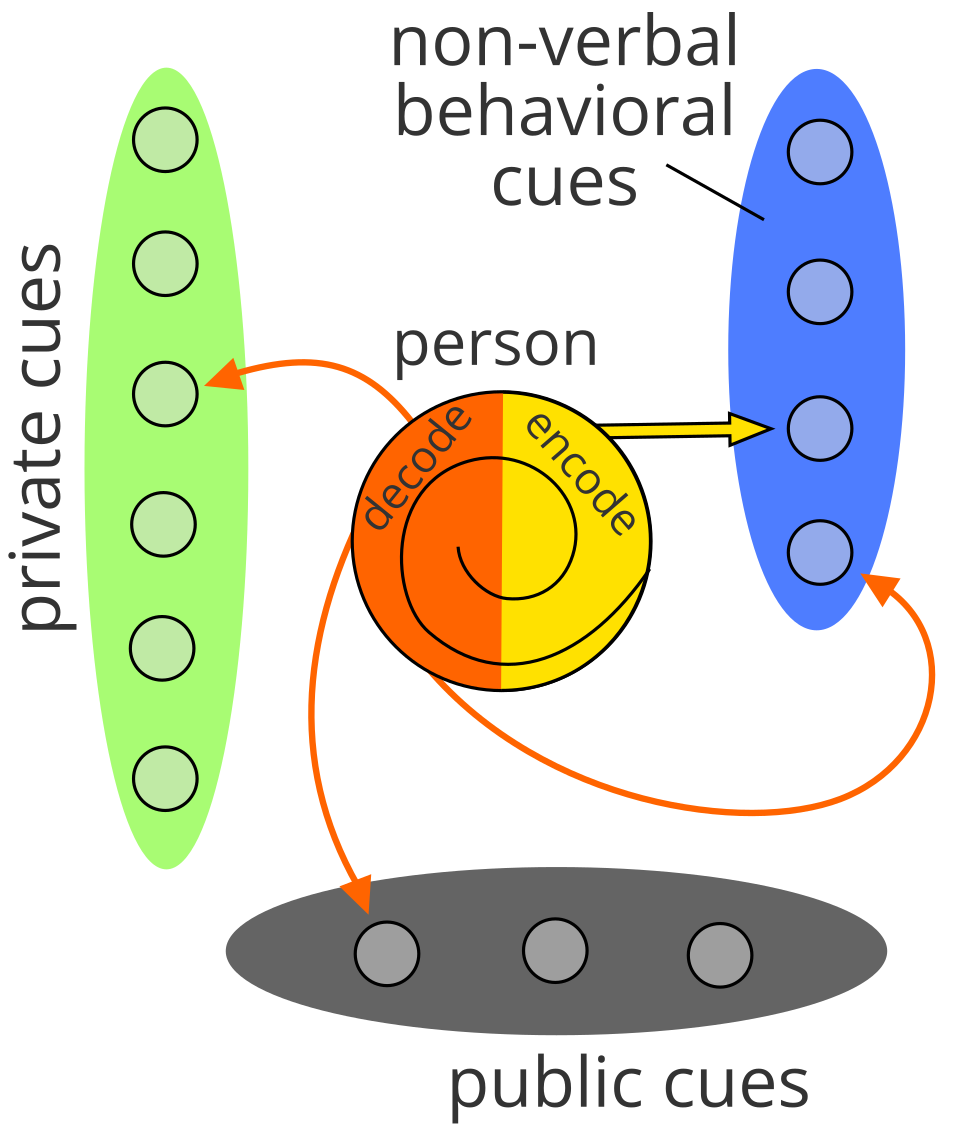
\includegraphics[width=0.9\textwidth]{barnlund_intera_personal.png}
            \end{figure}
        
        \subsection{Interpersonal}
            \seeherefooter{https://en.wikipedia.org/wiki/Barnlund\%27s_model_of_communication#Interpersonal_model}
            \begin{figure}[H]
                \centering
                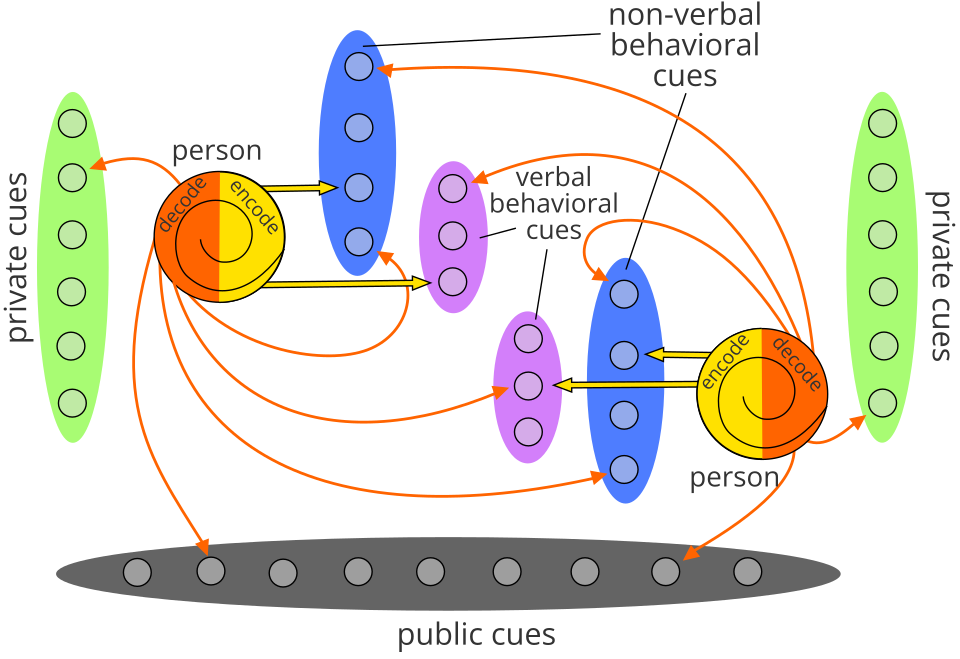
\includegraphics[width=0.9\textwidth]{barnlund_interpersonal.png}
            \end{figure}
            
            \bibliographystyle{plainnat}
            \bibliography{/home/donkarlo/Dropbox/repo/nd_shared_research/bibliography/bibliography.bib}
\end{document}